\chapter{Patched QTCI}
\label{chap:patching}

We've come now to the original part of this manuscript. In \prettyref{chap:QTCI} we introduced the state-of-the art implementation of the (Quantics) Tensor Cross Interpolation algorithm. We have briefly illustrated the capabilities of this numerical method through several simple examples, which have also been demonstrated in a more thorough manner in other studies \cite{Fernandez2022, Fernandez2024,
Ritter2024, Jolly2024, Sakurai2025, Oseledets2010, Dolgov2020}. Nevertheless, the final section of the previous chapter highlighted a few shortcomings of the standard implementation, particularly when dealing with more ill-defined cases. 

Here we present a more structured solution to these shortcomings than the one proposed in \prettyref{sec:TCIFallbacks} above, based on a \textit{``divide and conquer''} variant of the standard QTCI. Similar d.\&c. approaches have already been investigated in other tensor-focused works, including the use of an SVD-based Quantics Tensor Train (QTT) method for approximating many-body correlation functions \cite{Hiroshi2023, Murray2024}, and tensor compression techniques employing standard and High-Order Singular Value Decomposition (HOSVD) within adaptive or greedy frameworks \cite{Ehrlacher2021, FuenteRuizPhDThesis, Ehrlacher2022}. Our novel implementation of this method -- ``standing on the shoulder of these giants'' --  exploits the  advantages of TCI and performs TCI tensor compression and function approximation in a \textit{patched} way. 

This new version of the TCI algorithm, which we will refer to as \textit{patched (Quantics) Tensor Cross Interpolation} -- or \textit{patched (Q)TCI} -- distributes the workload of the cross approximation by adaptively splitting the configuration domain and uses the rank of the temporary TT cross approximation as trigger parameter for the splitting. We will show that this \textit{patching} technique helps reduce the computational demand of TCI when attempting to represent narrow peaked, multi-dimensional functions, both in memory requirements and CPU times. 

The upcoming chapter will be structured as follows: \prettyref{sec:patchAlg} covers all the technical and mathematical details about the patched QTCI routine and \prettyref{sec:patchingCost} discusses the estimated scaling of computational resources for the algorithm, while also adressing some its weaknesses.

\section{The algorithm}
\label{sec:patchAlg}

Patched Quantics Tensor Cross Interpolation (pQTCI) is an adaptive partitioning method \cite{Deng2008} based on rank-revealing cross approximation for high-dimensional tensors. Cross interpolation represents only a subroutine for our algorithm, hence, we will assume that the reader is familiarized with all TCI's functionalities (cf. \prettyref{chap:QTCI} and Ref. \cite{Fernandez2024} otherwise). Since it is built upon the TCI framework, pQTCI also falls within the class of \emph{rank‑revealing} algorithms introduced in \prettyref{def:rkralg}.

Given a high dimensional tensor $\mT$ with hidden low-rank structure and desirably -- but not necessarily -- very localized features in configurational space (\textit{i.e.} only for a small subset of $\bsigma$, $\mT_{\bsigma}$ is non-trivial) as input, pQTCI returns a \textit{collection} of TT unfoldings as output, that, when resummed, approximate the tensor $\mT$ on its whole domain. Let us dive into the prerequisites needed for the construction of pQTCI.


\subsection{Element-wise addition of TTs}
An indispensable piece to assemble the pQTCI algorithm is the TT summation operation. Consider the following definition
\begin{definition}[Direct sum]
	The {\normalfont \textbf{direct sum}} of $N$-dimensional tensors $X_{\bsigma} \in \mathds{K}^{d_1 \times d_2 \times \cdots d_N}$ and $Y_{\bsigma'} \in \mathds{K}^{d'_1 \times d'_2 \times \cdots d'_N}$ is defined by 
	\begin{equation}
		Z_{\bsigma''} = X_{\bsigma} \oplus Y_{\bsigma'} \in \mathds{R}^{(d_1+d'_1) \times (d_2+d'_2) \times \cdots (d_N+d'_N)}
	\end{equation}
	with entries
	\begin{equation}
		Z_{\sigma''_1, \dots, \sigma''_N} = \begin{cases}
			X_{\sigma''_1, \dots, \sigma''_N} & \text{if}\ 1\leq \sigma''_n \leq d_n \;\forall n\\
			Y_{\sigma''_1-d_1, \dots, \sigma''_N-d_N} & \text{if}\ d_n + 1\leq \sigma''_n \leq d_n + d'_n \;\forall n\\
			0 & \text{otherwise}.
		\end{cases}
	\end{equation}
\end{definition}
A special case of the direct sum of two tensors is the so-called \textit{partial direct sum} $\boxplus$ \cite{Lee2018}. A partial direct sum of two tensors $X_{\bsigma} \in \mathds{K}^{d_1 \times d_2 \times \cdots d_n \times d_{n+1} \times \cdots d_N}$ and $Y_{\bsigma'} \in \mathds{K}^{d'_1 \times d'_2 \times \cdots d'_n \times d_{n+1} \times \cdots d_N}$ is defined as 

\begin{equation}
	Z_{\bsigma''} = X_{\bsigma}\boxplus Y_{\bsigma'} \in \mathds{K}^{(d_1+d'_1) \times (d_2+d'_2) \times \cdots (d_n+d'_n) \times d_{n+1} \times \cdots d_N}
\end{equation}

where $Z_{\bsigma''}$, by means of the slicing operation introduced in \prettyref{eq:Tslices}, has subtensors

\begin{equation}
	Z_{(i''_n \oplus j_{n+1})} = X_{(i_n \oplus j_{n+1})} \oplus Y_{(i'_n \oplus j_{n+1})} \quad \forall j_{n+1} \in \mathds{J}_{n+1}\; \text{fixed}.
\end{equation}
The partial direct sum of $X_{\bsigma}$ and $Y_{\bsigma}$ is a direct sum performed pairwise between all the subtensors of the two addends, obtained from fixing the indices not included in the sum operation to the same value in both $X$ and $Y$.

Given now two $\mL$-dimensional tensor trains, $\widetilde{A}_{\bsigma}$ and $\widetilde{B}_{\bsigma}$\footnotemark,

\footnotetext{We use $\ \widetilde{}\ $ to refer to a generic MPS or TT unfolding (cf. \prettyref{chap:QTCI}).}

\begin{align}  
	\widetilde{A}_{\bsigma}
 &= A_1 A_2 \cdots A_\mL = \raisebox{-5.5mm}{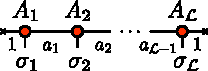
\includegraphics[scale=0.95]{figures/ATensorTrain.pdf}}, \\[6pt]
 \widetilde{B}_{\bsigma}
 &= B_1 B_2 \cdots B_\mL = \raisebox{-5.5mm}{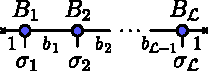
\includegraphics[scale=0.95]{figures/BTensorTrain.pdf}}
\end{align}
their element-wise sum $\widetilde{C}_{\bsigma} =  \widetilde{A}_{\bsigma} + \widetilde{B}_{\bsigma}$ is still a tensor trained shaped as
\begin{equation}
	\label{eq:TensorTrainsSum}   
	\widetilde{C}_{\bsigma}
 = \bigr[A_1 \boxplus B_1 \bigl]\bigr[A_2  \boxplus B_2 \bigl]\cdots \bigr[A_\mL \boxplus B_\mL \bigl] = \raisebox{-5.5mm}{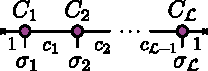
\includegraphics[scale=0.95]{figures/CTensorTrain.pdf}},
\end{equation}
where the partial sum between $A$'s and $B$'s sitetensors is performed by fixing the sites indices $\sigma_\ell$, and results in

\begin{equation}
	C_1^{\sigma_1} =
	\begin{bmatrix}
	  A_1^{\sigma_1} & B_1^{\sigma_1} \\
	\end{bmatrix},\quad C_\ell^{\sigma_\ell} =
	\begin{bmatrix}
	  A_\ell^{\sigma_\ell} & 0 \\
	  0 & B_\ell^{\sigma_\ell}
	\end{bmatrix},\quad C_\mL^{\sigma_\mL} = \begin{bmatrix}
		A_\mL^{\sigma_\mL} \\[6pt]
		B_\mL^{\sigma_\mL} 
	  \end{bmatrix}.
	\label{eq:siteTenosorsTTSum}  
\end{equation}

The new internal bonds $c_\ell$ are dependent on the original bonds, in fact $a_\ell = c_\ell$ and $b_\ell = c_\ell - \chi^A_\ell$. Hence, the bond dimensions\footnotemark \;of the sum are also additive \textit{w.r.t} to the bond dimensions of its addends

\begin{equation}
	\chi^C_\ell = \chi^A_\ell + \chi^B_\ell.
\end{equation}

\footnotetext{The bond dimension at site $\ell$ ($1\leq\ell<\mL$) is defined as the number of columns of the $\ell^{\text{th}}$ site tensor, when $\sigma_\ell$ is fixed to a specific value. }

\subsection{Tensor subdomain projection}
The second requirement needed to construct patched QTCI is, what we will refer to as, the \textit{subdomain projection} operation. 

Consider a $\mL$-dimensional tensor $\Psi_{\bsigma}$; $\Psi_{\bsigma}$ can be interpreted as the collection of coefficients of a generic quantum state $\ket{\Psi}$, when represented on a specific basis of the Hilbert space it belongs to, as
\begin{align}
	\ket{\Psi} = \Psi_{\bsigma}\ket{\bsigma} &= \Psi_{\sigma_1,\sigma_2,\dots,\sigma_\mL} \ket{\sigma_1}, \ket{\sigma_2}\dots \ket{\sigma_\mL} \\[6pt]
	\nonumber &= \raisebox{-5mm}{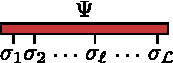
\includegraphics[scale=0.95]{figures/LTensor_ell_leg.pdf}}\; \footnotemark.
\end{align}
\footnotetext{By abuse of notation we identify the tensor $\Psi_{\bsigma}$ with the quantum state $\ket{\Psi}$.}
In the same way, its MPS unraveling
\begin{align}
	\label{eq:quantumMPS}
	\ket{\Psi} = \widetilde{\Psi}_{\bsigma}\ket{\bsigma} &=  [M_1^{\sigma_1}]_{1 m_1}\ket{\sigma_1}  [M_2^{\sigma_2}]_{m_1 m_2} \ket{\sigma_2} \cdots  [M_\mL^{\sigma_\mL}]_{m_{\mL -1} 1} \ket{\sigma_\mL} \\[6pt]
	\nonumber &= \raisebox{-5mm}{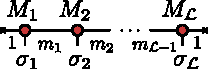
\includegraphics[scale=0.95]{figures/MTensorTrain.pdf}}.
\end{align}

If we restrict the configuration space to a subset space where $\ket{\sigma_\ell}$ is fixed to a specific basis vector $\ket{p_\ell}$, the corresponding subtensor representation of such a subspace state $\ket{\Psi^{p_\ell}}$ would be  

\begin{align}
	\label{eq:tensorSlice}
	\nonumber \ket{\Psi^{p_\ell}} &= \Psi_{\sigma_1,\dots,\sigma_{\ell -1}, p_\ell, ,\sigma_{\ell +1}, \dots, \sigma_\mL} \ket{\sigma_1},\dots,\ket{\sigma_{\ell -1}},\ket{p_\ell},\ket{\sigma_{\ell +1}},\dots, \ket{\sigma_\mL}\\[6pt]
	&= \Psi^{p_\ell}_{\sigma_1,\dots,\sigma_{\ell -1},\sigma_{\ell +1}, \dots, \sigma_\mL} \ket{\sigma_1},\dots,\ket{\sigma_{\ell -1}},\ket{p_\ell},\ket{\sigma_{\ell +1}},\dots, \ket{\sigma_\mL}\\[6pt]
	\nonumber &= \raisebox{-5mm}{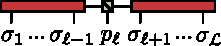
\includegraphics[scale=0.95]{figures/PsiPSubtensor.pdf}} =\; \raisebox{-4.5mm}{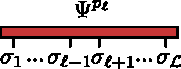
\includegraphics[scale=0.95]{figures/PsiSubtensor.pdf}}.
\end{align}

This procedure resembles a quantum projection, \textit{i.e.} $\ket{\Psi^{p_\ell}} = \ket{p_\ell}\braket{p_\ell|\Psi}$, ergo the \textit{projection} labeling of the operation. 
For now, the object \raisebox{-1.5mm}{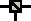
\includegraphics[scale=0.95]{figures/ProjectionTensor.pdf}} is only used as a placeholder to relate our subtensor of interest $\Psi^{p_\ell}_{\sigma_1,\dots,\sigma_{\ell -1},\sigma_{\ell +1}, \dots, \sigma_\mL}$  to the original configuration space of the full tensor $\Psi_{\bsigma}$, but has otherwise no other meaning. Indeed, within the $\ket{p_\ell}$-subspace, $\ket{\Psi^{p_\ell}}$ is completely defined by the $\mL - 1$ indices $(\sigma_1,\dots,\sigma_{\ell-1},\sigma_{\ell+1},\dots,\sigma_\mL)$. The \raisebox{-1.5mm}{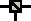
\includegraphics[scale=0.95]{figures/ProjectionTensor.pdf}} items act as \textit{slicing} or \textit{projection} operators that limit us to the subsector of $\Psi_{\bsigma}$ where the $\ell^{\text{th}}$ index is fixed to $p_\ell$. It is trivial to deduce that
\begin{equation}
	\ket{\Psi} = \sum_{p_\ell = 1}^{d_\ell} \ket{\Psi^{p_\ell}},
\end{equation}
and, thus,

\begin{equation}
	\raisebox{-5mm}{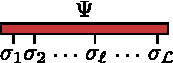
\includegraphics[scale=0.95]{figures/LTensor_ell_leg.pdf}} = \sum^{d_\ell}_{p_\ell=1}\ \raisebox{-5.4mm}{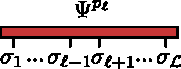
\includegraphics[scale=0.95]{figures/PsiSubtensor.pdf}}.
	\label{eq:subTensorSum}
\end{equation}

Inside a specific $\ket{p}$-subspace we can perform a TT approximation of the subtensor $\Psi^p$ as follows

\begin{equation}
	\widetilde{\Psi}^{p_\ell} = \raisebox{-5.5mm}{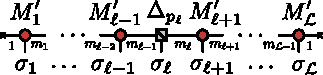
\includegraphics[scale=0.95]{figures/ProjTensorTrain.pdf}} 
\end{equation}
wherein we generalized \raisebox{-1.5mm}{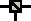
\includegraphics[scale=0.95]{figures/ProjectionTensor.pdf}} to be local state dependent in the following manner

\begin{equation}
\raisebox{-4.5mm}{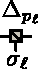
\includegraphics[scale=0.95]{figures/ProjectionTensor_lLabel.pdf}} = \begin{cases}
		[\mathds{1}]_{m_{\ell-1},m_\ell} & \text{if } \sigma_\ell = p_\ell \\
		[0]_{m_{\ell-1},m_\ell} & \text{otherwise},
	\end{cases}
\end{equation}
with bonds $m_{\ell-1}$ and $m_{\ell}$ of same dimension and where $0_{m,n}$ denotes the element $(m,n)$ of the zero matrix.
From \prettyref{eq:subTensorSum} we can recognize that 

\begin{equation}
	\Psi_{\bsigma} \simeq \sum_{p_\ell = 1}^{d_\ell} \widetilde{\Psi}^{p_\ell} =  \sum_{p_\ell = 1}^{d_\ell} \raisebox{-5.5mm}{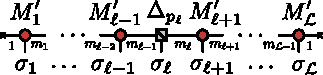
\includegraphics[scale=0.95]{figures/ProjTensorTrain.pdf}}
\end{equation}
where the first equality reflects the error associated with an arbitrary MPS approximation and the sum is performed according to the element-wise TT addition described by \prettyref{eq:TensorTrainsSum} in the section above. Without loss of generality, the same line of reasoning can be applied to smaller subspaces in such a way
\begin{equation}
	\Psi_{\bsigma} \simeq \widetilde{\Psi}^{+}_{\bsigma} = \sum_{p_{\ell_1}= 1}^{d_{\ell_1}} \cdots \sum_{p_{\ell_N}= 1}^{d_{\ell_N}} \widetilde{\Psi}^{p_{\ell_1},\dots,p_{\ell_N}}
	\label{eq:NslicesSum}
\end{equation}
taking $(\ell_1, \dots, \ell_N) \in \{1,\dots, \mL\}^{N(\leq \mL)}$ ($\ell_i \neq \ell_j$ for every $i\neq j$) without any specific order constraint. $\widetilde{\Psi}^{+}_{\bsigma}$ is good approximation of the original tensor $\Psi_{\bsigma}$.

\subsection{The Patching scheme}
Having laid out all the necessary ingredients, we now return to detailing our patched (Q)TCI algorithm. 
Consider a generic tensor $\mT_{\bsigma}$ and its TCI approximation $\widetilde{\mT}_{\bsigma}$. As noted in \prettyref{sec:TCIFallbacks}, when the tensor $\mT$ exhibits sharply localised structures, its compression $\widetilde{\mT}$ can be made more memory-efficient by adopting a \textit{divide-et-impera} approach. Nevertheless, although the naive domain-splitting approach outlined in \prettyref{sec:TCIFallbacks} proved functional, it provided no means of numerical control and presumed that both the location and spatial extent of the tensor’s relevant features were known a priori. Such ideal conditions are rarely encountered in real-world applications, particularly when the tensor $\mT$ stems from complex computations that estimate unknown variables. However, the preceding example shows that memory usage for a (local) TT approximation is effectively characterised by its bond dimensions $\chi_\ell$—specifically, by the maximum bond dimension $\chi$. Recognizing this allows us to devise a more intelligent, adaptive, and general solution to the compression of tensors presenting sharp localized features.

The standard TCI implementation provided by \texttt{TCI.jl} \cite{TensorCrossInterpolation.jl}, as illustrated in Listing \ref{code:crossinterpolate2}, offers a mechanism to control the bond dimension of the approximation. Specifically, setting the input variable \texttt{maxbonddim} within \texttt{crossinterpolate2} constrains the size of the pivot lists $\mathcal{I}\ell$ and $\mathcal{J}\ell$, thereby restricting the bond dimensions $\chi_\ell$ of the resulting MPS. Although this strategy effectively reduces the memory footprint of the TCI approximation, it also hampers the convergence of the algorithm. Consequently, to ensure convergence, the approximation domain must be suitably reduced. 

We partition the approximation domain through \textit{subdomain projection} operation—or tensor \textit{slicing}- as detailed in the previous section. Once the original tensor has been decomposed into subtensors, hereafter called \textit{patches} \footnotemark, we run TCI on each patch separately. Working on these reduced domains improves the likelihood of convergence since each patch explores a much smaller configuration space, even when the bond dimension is capped at the prescribed threshold $\chi_{\text{patch}}$, a bound that will then not be reached.
This whole procedure can be repeated iteratively and adaptively, as shown in \prettyref{fig:patchingAlg}. We shall refer to this routine as the \textit{patching scheme}, or simply \textit{patched TCI}.
The algorithm proceeds as follows:
\footnotetext{Henceforth, the term \textit{patch} will denote both the subtensor $\mT^{p_1,\dots,p_\ell}$ and its TT-unfolded form $\widetilde{\mT}^{p_1,\dots,p_\ell}$.}
\begingroup
\renewcommand{\labelenumi}{(\arabic{enumi})}
\begin{enumerate}
	\item Start the standard TCI routine on the full tensor $\mT_{\bsigma}$ either from
	\begin{itemize}
		\item a random configuration $\hat{\sigma}$ or
		\item a tailored set of global pivots, if prior information about local features of $\mT$ is available.
	\end{itemize}
	The rank reveal of the tensor train $\widetilde{\mT}$ is constrained by the prescribed limit $\chip$. If $\widetilde{\mT}_{\bsigma}$ converges, the algorithm terminates. 
	\item If convergece is not reached, slice $\mT_{\bsigma}$ along its first index to produce subtensors 
	$$\mT^{p_1}\quad \forall p_1 \in \{1,\dots,d_1\}\quad \text{(cf. \prettyref{eq:tensorSlice}).}$$
	\item Use the pivot lists $\mathcal{I}_\ell$ and $\mathcal{J}_\ell$ from the preceding (failed) TT to form new global pivots: $\hat{\sigma} = i_\ell \oplus j_{\ell +1}$, with $i_\ell \in \mathcal{I}_\ell$, $j_{\ell+1} \in \mathcal{J}_{\ell +1}$. 
	A pivot $\hat{\sigma}$ is assigned to subtensor $\mT^{p_1}$ whenever its first component satisfies $\hat{\sigma}_1 = p_1$.
	\item Compress each subtensor $\mT^{p_1}$ with TCI  (bond dimension is still capped at $\chip$) over the reduced cofiguration domain $(\sigma_2, \dots, \sigma_\mL)$.  Store all the converged \textit{patches} $\widetilde{\mT}^{p_1}$; discard those that fail to converge. 
	\item For every unconverged subtensor $\mT^{p_1}$, slice further along the next index to obtain $\mT^{p_1, p_2}\  \forall p_2\in {1,\dots,d_2}$. Build the next set of global pivots subject to $\hat{\sigma}_1 = p_1$ and $\hat{\sigma}_2 = p_2$.
	\item Repeat step (4)-(5), recursively increasing the slicing depth, until no \textit{patches} remain to be converged. 
\end{enumerate}
\endgroup

\begin{figure}[ht!]
	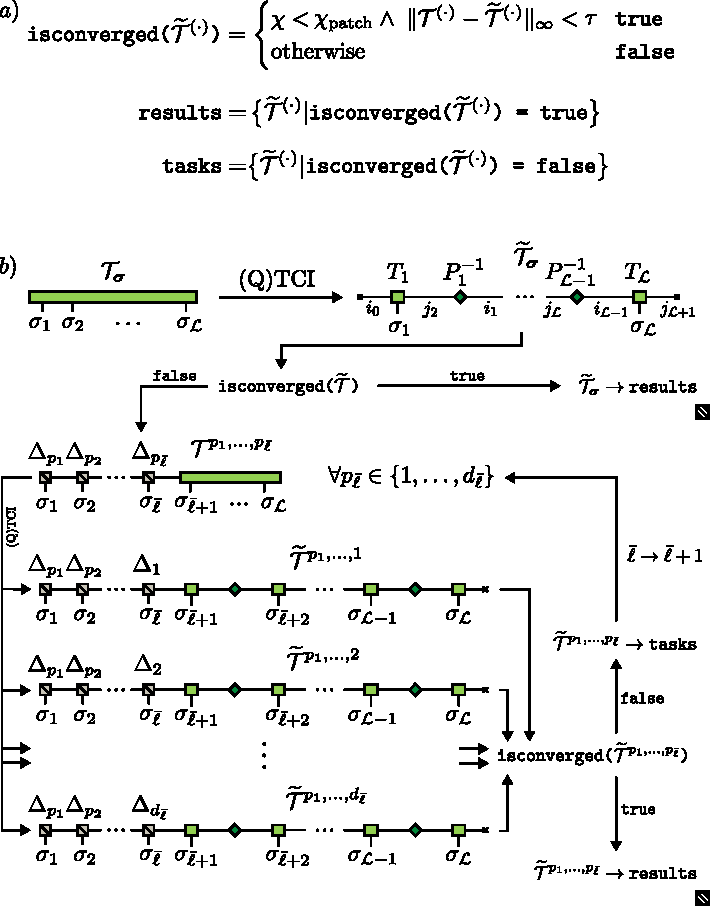
\includegraphics{figures/PatchingAlgorithm.pdf}
	\caption{Flowchart of the patched TCI algorithm. $(a)$ Convergence criterion for the subtensors $\widetilde{\mT}^{p_1,\dots,p_{\bar \ell}}$ -- or \textit{patches} -- defined by the parameters $\chi_{\text{patch}}$ and $\varepsilon$, and the two sets of subtensors that have already converged -- \texttt{results} -- and those yet to converge  -- \texttt{tasks}. $(b)$ Flowchart of the \textit{patching scheme}. The TCI approximation is adaptively decomposed into smaller computations through \textit{slicing} (cf. \prettyref{eq:tensorSlice}). Each subtensor is TCI compressed within the smaller domain. The converged \textit{patches} are added to \texttt{results}, the yet-to-converge ones to \texttt{tasks}. The algorithm terminates -- 
\includegraphics[scale=0.95]{figures/TerminalSquare.pdf} -- when \texttt{tasks} is empty. We refer the reader to the main manuscript for additional details.}
	\label{fig:patchingAlg}
\end{figure}

A series of remarks are in order. The output result of the algorithm seems to be a collection of tensor trains of the form 
\begin{equation}
	\raisebox{-4.5mm}{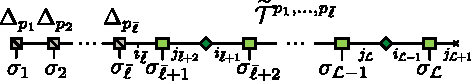
\includegraphics{figures/PatchTensorTrain.pdf}}
	\label{eq:patchedTT}
\end{equation}
where both the \textit{prefix} indices $(p_1,\dots,p_{\bar{\ell}}) \in \mathds{I}_{\bar{\ell}}$ and the length of the prefix -- the \textit{paching level} -- $\bar{\ell} \in \{1,\dots,\mL\}$ can take very different values. Nevertheless, two conditions are respected from our implementation:
\begin{itemize}
	\item since any subtensor that is further subdivided has its non-convergent TT approximation discarded, all pairs of index prefixes satisfy
	\begin{equation}
		(p_1,\dots,p_{\bar{\ell}_1}) \nsubseteq (p_1,\dots,p_{\bar{\ell}_2}) \quad \forall\, \bar{\ell}_1, \bar{\ell}_2
	\end{equation}
	 Consequently, the patched-TCI procedure produces TT approximations $\widetilde{\mT}^{p_1,\dots,p_{\bar \ell}}$ that are strictly \textit{non-overlapping} (\textit{disjointed}) in configuration space; 
	\item the collection of TTs of the form in \prettyref{eq:patchedTT}, in order to constitute a good approximation for the full tensor $\mT_{\bsigma}$, satisfies the condition  
	\begin{equation}
		\mT_{\bsigma} \approx \sum_{\widetilde{T}^{(\cdot)} \in \texttt{results}} \widetilde{\mT}^{(\cdot)}.
	\end{equation}
	and we can therefore resum them to a single tensor train $\widetilde{\mT}^{+}_{\bsigma}$, similar to what we did in \prettyref{eq:NslicesSum}. $\widetilde{\mT}^{+}_{\bsigma}$ is a good TT representation of $\mT$. However due to the adaptivity of pQTCI, differently from \prettyref{eq:NslicesSum}, here we might be presented with a series of \textit{patches} $\widetilde{\mT}^{p_1,\dots,p_{\bar \ell}}$ with prefixes $(p_1,\dots,p_{\bar \ell})$ of different lengths ${\bar \ell}$; nonetheless, this intricacy does not affect the TT sum operation.
\end{itemize}

In \prettyref{fig:patchingAlg} we displayed a version of the patched TCI where the tensor is sliced sequentially starting from the first index $\sigma_1$ of the tensor $\mT$. As pointed out already, this constraint is not required to obtain a meaningful outcome from the algorithm.
% (we refer the reader to \prettyref{app:patchordering} for details about the impact of the \textit{prefix ordering} -- or \textit{patch ordering} -- on the approximation)
The \textit{prefix} of each subtensor $\mT^{p_1,\dots,p_{\bar \ell}}$ -- that indicates to which slice of $\mT$ it corresponds to -- can be taken randomly, in an exclusive manner, from the set of tensor indices $\{\sigma_1,\dots,\sigma_\mL\}$ (considered labels in this context).

Let us consider now the specific case when we intend to TT approximate a multi-variate function, call it $f(\boldsymbol{x})$. \prettyref{sec:TCIalgorithm} taught us that, when we intend to properly resolute all the relevant features of $f$, it is a clever choice to numerically represent it as a tensor utilizing the quantics discretization (with $\mR$ bits per spatial dimention $x_i$): in fact, the discretization error of the approximation decreases exponentially by increasing $\mR$ only linearly. 

Assume now that $f$ is characterized by narrow peaks sparsely distributed across its domain. Its tensor representation $\mF_{\bsigma} = f(\boldsymbol{x}(\bsigma))$ inherits the same structure. When we apply the patched TCI procedure to $\mF_{\bsigma}$, the scale separation introduced by the quantics format (where $\sigma_{\ell(n,r)} \to 2^{-r}$ length scale) implies that each patch $\widetilde{\mF}^{p_1,\dots,p_{\bar \ell}}$ simply captures $f(\boldsymbol{x}(\bsigma))$ restricted to a distinct sub-region of the original domain.
\prettyref{fig:patchSubdivision} makes the idea clearer for a bivariate function.
The tensor $\mF$ is indexed by scale: for example, with an interleaved 2-D ordering, the first two indices $\sigma_1$ and $\sigma_2$ encode the resolution $2^{-1}$ in the $x$- and $y$-directions. Fixing these two indices—i.e., taking the corresponding slice—yields a smaller subtensor that represents $f$ on one quarter of the domain (see the second panel on the right in \prettyref{fig:patchSubdivision}). This motivates our previous terminology: we call each such subtensor slice a \textit{patch}.
\begin{figure}[ht!]
	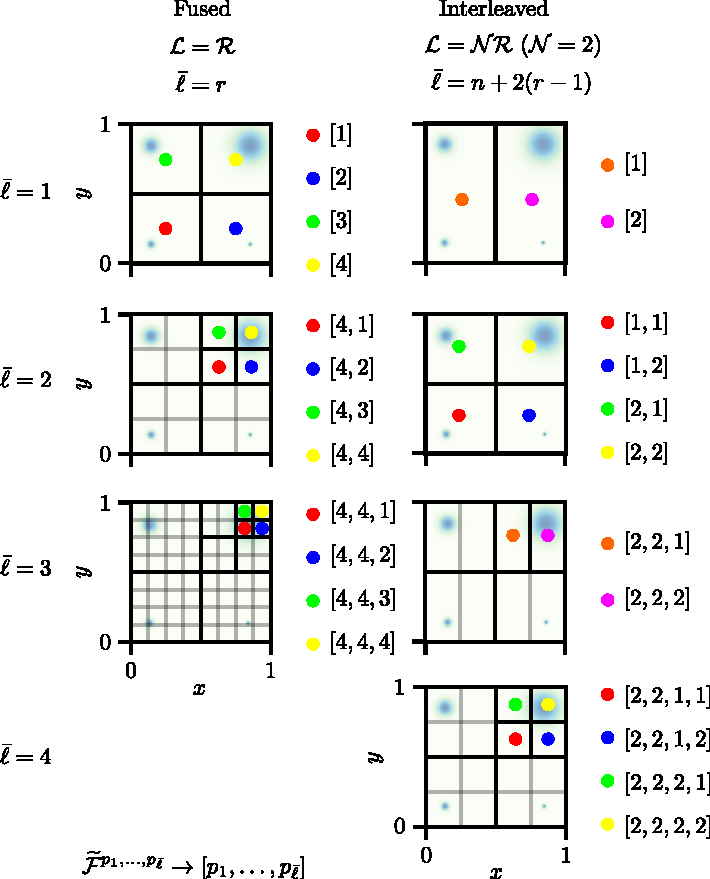
\includegraphics{figures/PatchDivision.pdf}
	\caption{Subdivision of a two-dimensional domain caused by the QTCI patching scheme. For clarity, we label each patch $\widetilde{\mathcal F}^{p_1,\dots,p_{\bar\ell}}$ by its prefix $\bigl[p_1,\dots,p_{\bar\ell}\bigr]$. We consider both fused and interleaved index ordering for the TTs $\widetilde{\mathcal F}^{p_1,\dots,p_{\bar\ell}}$. Coloured dots show the region represented by each patch, and only selected patches are displayed up to a \textit{patching level} $\ellb=4$. Faded grid lines suggest how the remaining parts of the domain could be further split whenever the adaptive-convergence criterion of the patched QTCI algorithm calls for it.}
	\label{fig:patchSubdivision}
\end{figure}

Patched QTCI refines the domain more aggressively in regions where the target function $f$ exhibits higher complexity. Areas that contain sharp, localised peaks incur a larger memory footprint, driving up the tensor-train rank $\chi$. Panel $(a)$ of \prettyref{fig:patchTree} illustrates this effect for a generic, single-peaked bivariate function. As noted earlier, patched TCI returns a collection of TT representations that are mutually disjoint in configuration space; in the context of pQTCI this means that the resulting set of patches forms a non-overlapping cover of the entire domain of $f$. Panel $(b)$ shows how this cover is built: the algorithm traverses the patch tree and, for each slice $\widetilde{\mF}^{p_1,\dots,p_{\bar\ell}}$, checks the stopping criteria: 
\begin{equation}
	\| \mF^{(\cdot)} - \widetilde{\mF}^{(\cdot)} \| < \varepsilon \quad \text{and} \quad \chi < \chip.
	\label{eq:patchConvergence}
\end{equation}
adaptively refining only those slices that violate either boundary. The total number of red colored leaves in \prettyref{fig:patchTree} is the number of patches, $\Np$, for a specific approximation.
\begin{figure}[ht!]
	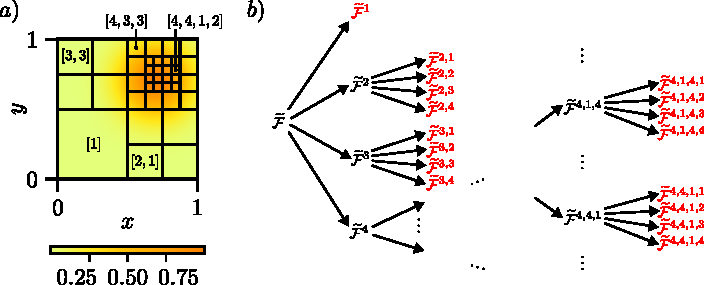
\includegraphics{figures/PatchingTree.pdf}
	\caption{Patched QTCI applied to the TT approximation of a bivariate function. $a)$ The domain is adaptively split, yielding finer cells where the function is more intricate. $b)$ Hierarchical tree that records the patch refinement: each tensor slice is attached to its parent, and the red leaves mark the final subtensors produced and kept by pQTCI. }
	\label{fig:patchTree}
\end{figure}

\section{Computational Costs and Scaling}
\label{sec:patchingCost}


In many practical settings, applying standard Tensor Cross Interpolation (TCI) directly to large, feature-sparse tensors is wasteful: a lot of the computational effort is spent on regions that do not influence the final accuracy. Moreover,
since all TCI algorithms involve sampling, none of them is fully immune against missing some features of the tensor of interest, as already discussed above. Patched QTCI addresses these issues by adaptively dividing the tensor into small, targeted patches and capping the bond dimension in each local solve. The goal is to concentrate resources only where the data truly demands high resolution, while discovering the interesting regions during the process, thereby reducing both memory traffic and run-time.

At first sight, the patched (Q)TCI algorithm shown in \prettyref{fig:patchingAlg} appears to burden the original TCI routine with considerable overhead: in the worst-case, \texttt{crossinterpolate2} is invoked on the order of $\mathcal{O}\bigl(d^{\bar\ell}\bigr)$ times, where $\bar\ell$ is the deepest patching level reached (assuming a uniform subdivision and ignoring adaptivity).

In practice, however, patched QTCI can run faster than the plain TCI workflow. Every call to \texttt{crossinterpolate2} is restricted by the bond-dimension cap $\chi_{\text{patch}}$, so each local TCI solve is far cheaper than a full-rank solve on the entire tensor $\mT$. Only when we reach patch spatial dimension containing features we are able to approximate within a bond dimension of $\chip$ then the TCI procedure runs to its full extent, reaching convergence. 

The preceding discussion makes it clear that both the total number of resulting patches, $\Np$, and relative computational resources expenditure, are governed largely by the bond-dimension cap assigned to each patch, $\chi_{\text{patch}}$. 

\subsection{Runtime \& Memory vs. $\chip$}

To estimate actual resource usage of pQTCI, we begin with a theoretical analysis (empirical fits are presented later in \prettyref{chap:results}). 
Consider a generic Tensor-Train $\widetilde{\mT}$ of the form given in \prettyref{eq:quantumMPS} whose maximum bond dimension is $\chi$. When $\widetilde{\mT}$ is constructed by successive SVD unfoldings of the full tensor $\mT$, truncating each SVD at the rank $\chi$ \cite{vonDelftTNNotes, Fannes1992, tensornetwork.org}, the bond dimension along the chain typically evolves  as illustrated in \prettyref{fig:typicalBondDim}.

\begin{figure}[ht!]
	\centering
	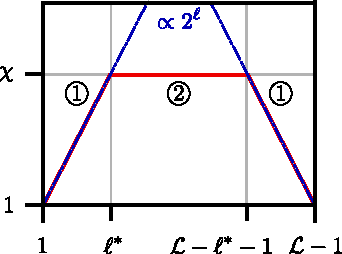
\includegraphics{figures/TypicalBondDims.pdf}
	\caption{Generic $\chi$ truncated MPS bond dimension evolution.}
	\label{fig:typicalBondDim}
\end{figure}

A convenient way to gauge the memory footprint of a tensor-train approximation is to tally the total number of floating-point entries it contains. For each of the two TT splittings labelled \raisebox{.5pt}{\textcircled{\raisebox{-.9pt}{1}}} and \raisebox{.5pt}{\textcircled{\raisebox{-.9pt}{2}}} in \prettyref{fig:typicalBondDim} -- assuming all physical dimensions satisfy $d_\ell = d$ -- the parameter count is therefore

\begin{equation}
	\begin{aligned}
		N^{\raisebox{.5pt}{\tiny \textcircled{\raisebox{-0.6pt} {1}}}}_{\text{par}} &= 2 *\sum\limits_{\ell = 1}^{\ell^*} d^{2\ell}  \\[6pt]
		N^{\raisebox{.5pt}{\tiny \textcircled{\raisebox{-0.6pt} {2}}}}_{\text{par}} &= \sum\limits_{\ell = \ell^* + 1}^{\mL - \ell^* - 1} \chi^2d
	\end{aligned}
\end{equation}

Hence, the total number of parameters for a generic TT of this form is bounded by
\begin{equation} 
	N_{\text{par}} \lesssim 2 d^2 \frac{1 - \chi^2 }{1 - d^2} + \chi^2d (\mL - 2 \log_d \chi - 2). 
\end{equation}
Assume the worst-case scenario in which patched QTCI subdivides the entire domain into a lattice of equally ranked patches. After sequential slicing ($\sigma_1 \to \sigma_2 \to \cdots$), the procedure halts at \textit{patching level} ${\bar \ell}$, yielding a total number of patches $\Np$ all with rank $\chip$ and with bond dimension development as in \prettyref{fig:typicalBondDim}. The memory footprint of this final object would be 
\begin{equation}
	\begin{aligned}
		N_{\text{par}} &= \Np\, N_{\text{par}\times \text{patch}}\\
		N_{\text{par}\times \text{patch}} &\lesssim  2 d^2 \frac{1 - \chip^2 }{1 - d^2} + \chip^2d (\mL - \ellb - 2 \log_d \chip - 2).
	\end{aligned}
	\label{eq:patchMemoryEstimate}
\end{equation}

As in standard TCI (see \prettyref{tab:cost}), the memory footprint of patched QTCI grows with the square of the maximum bond dimension — here evaluated per patch — scaling as  
\begin{equation}
	\order\bigl(\Np \chip^2 d^2 \mL\bigr). 
	\label{eq:PatchMemoryScaling}
\end{equation}

A comparable reasoning yields an estimate for the runtime  of the patched QTCI routine. If a single, full-domain TCI run takes  $\order\bigl( \chi^3 d^2 \mL \bigr)$ CPU time, then the cumulative runtime of patched QTCI becomes
\begin{equation}
	t_{\text{patch}} \lesssim \chip^3 d^2 \sum_{\ell = 0}^{{\bar \ell}} d^\ell (\mL - \ell) \lesssim  \Np \chip^3 d^3 \mL,
\end{equation}
where we assumed $\mL \gg \ellb$ in the last inequality. This yields a runtime scaling for pQTCI of 
\begin{equation}
	\order\bigl(\Np \chip^3 d^3 \mL\bigr).
	\label{eq:PatchTimeScaling}
\end{equation}

Beyond the raw cost estimates, the analysis yields some useful thresholds: the patched scheme remains more memory- or time-efficient than standard TCI only if the total number of patches, $\Np$, stays below the corresponding bounds:

\begin{equation}
  \begin{tabular}{ccc}
    \cline{2-3}
      & \textbf{memory cost} & \textbf{CPU runtime} \\ \cline{2-3} \\[-6pt]
    $\Np\;<$ &
      $\displaystyle \frac{\chi^{2}}{\chi_{\text{patch}}^{2}}$ &
      $\displaystyle \frac{\chi^{3}}{d\chi_{\text{patch}}^{3}}$ \\[15pt]\cline{2-3}
  \end{tabular}
  \label{eq:chiPatchBound}
\end{equation}

The table above provides us with rough boundaries on $\Np$ for an optimal pQTCI approximation. In this particular context, $\chi$ is the rank of an analogous (Q)TCI compression with the same input tensor of p(Q)TCI

\subsection{Number of patches vs. $\chip$}
To explore the dependence of $\Np$ by the fixed parameter $\chip$, let us examine a concrete example, in particular let us revisit the function of \prettyref{eq:localFunc} with the following parameter changes (purely for visualization purposes)
\begin{equation}
	\label{eq:localFuncNewParams}
\begin{gathered}
	\boldsymbol{r}_{1} = ( 0.2, 0.2), \quad \boldsymbol{r}_{2} = ( 0.8, 0.8),\\[6pt]
	A_2 = 2\, A_1 = 10^4, \quad \sigma_1 = 2\, \sigma_2 = 10^{-1}, \quad k_1 = 2\, k_2 = 10^3. 	
\end{gathered}
\end{equation}

We restate the formula here for simplicity

\begin{equation*}
		f(\boldsymbol{r}) = A_1\,e^{-\frac{(\boldsymbol{r} - \boldsymbol{r}_1)^2}{2\sigma^2_1}} \sin(k_1\boldsymbol{r}) + A_2\,e^{-\frac{(\boldsymbol{r} - \boldsymbol{r}_2)^2}{2\sigma^2_2}} \sin(k_2\boldsymbol{r}). 
\end{equation*}
We discretize $f$ on the square domain $[0,1]^2$ into the tensor $\mF_{\bsigma} = f(\boldsymbol{r}(\bsigma))$, using interleaved or fused quantics representation. Applying the patched QTCI compression to $\mF$, while varying the bond-dimension cap $\chip$, let us track how the domain is adaptively partitioned and how the overall patch count $\Np$ changes with $\chip$. 
Lowering the bond-dimension cap $\chip$ in the patched QTCI algorithm forces each patch to converge on a progressively smaller portion of the configuration space. This behaviour is illustrated in \prettyref{fig:patchEvolution}. 

\begin{figure}[htbp]
	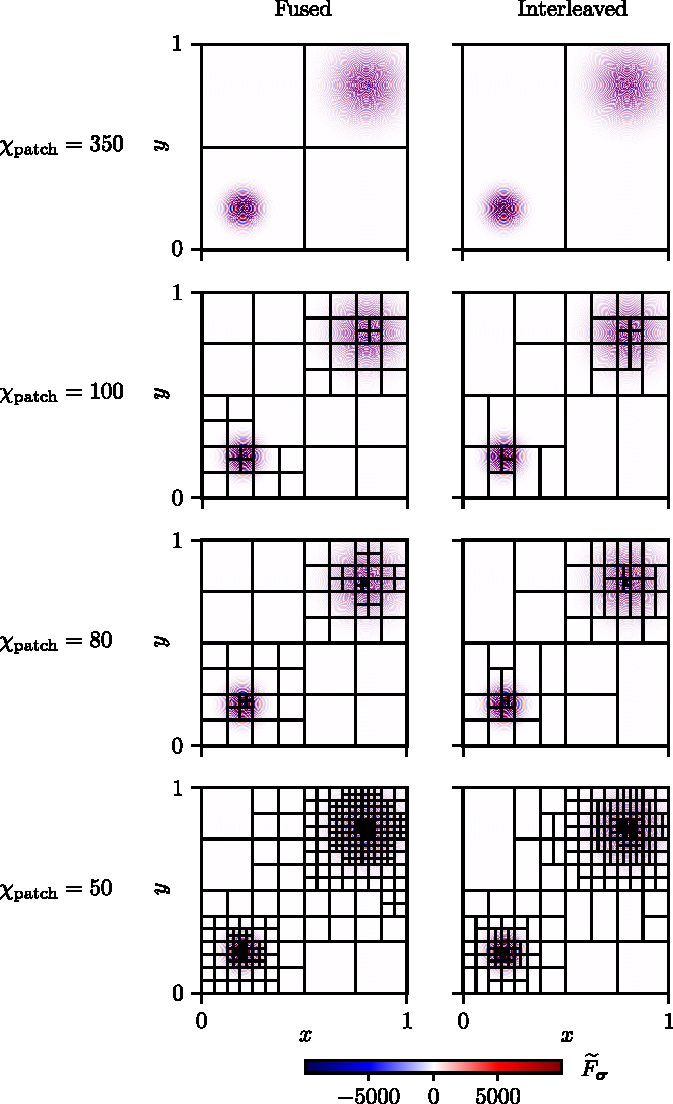
\includegraphics{figures/PatchEvolutionwithChi.pdf}
	\caption{Evolution of the adaptive partitioning of the bivariate function $f(\boldsymbol{r})$ domain (cf. \prettyref{eq:localFunc} and \prettyref{eq:localFuncNewParams}), due to pQTCI. Interleaved or fused orderin is utilized for the indices of the tensor $\mF_{\bsigma} = f(\boldsymbol{r}(\bsigma))$. Smaller maximum bond dimensions per patch $\chip$ render finer partitionings of the domain.}
	\label{fig:patchEvolution}
\end{figure}



In \prettyref{fig:patchEvolution} each coordinate is discretised with $\mR = 17$ bits--enough to resolve every feature of $f(\boldsymbol{r})$
f to a tolerance of $\varepsilon=10^{-7}$.
The total patch count $\Np$ depends sensitively on the chosen bond-dimension cap $\chip$
We can then understand that there exists a strond dependence of $\Np$ by $\chip$. From the memory estimate in \prettyref{eq:patchMemoryEstimate}, and assuming the overall parameter budget of the final approximation to stay roughly constant, we anticipate the following scaling law
\begin{equation}
	\Np \propto 1 / \chip^2. 
	\label{eq:scalingNpatchBonddim}
\end{equation}
In other words, halving the allowable bond dimension per patch would quadruple the number of patches required to achieve the same accuracy.
\prettyref{fig:NpatchvsChipatch} corroborates this scaling: it plots the patch count against the actual maximum bond dimension, $\chip^*$\footnotemark, attained by the most demanding patch in the pQTCI compression of $\mF_{\bsigma}$.
\footnotetext{The value of the bond dimension bound $\chip$ fixed by the user doesn't always correspond to the maximum bond dimension at which TCI converges within each patch. The largest of these maximum bond dimensions among all the patches is here referred to as $\chip^*$. }
\begin{figure}[htbp]
	\centering
	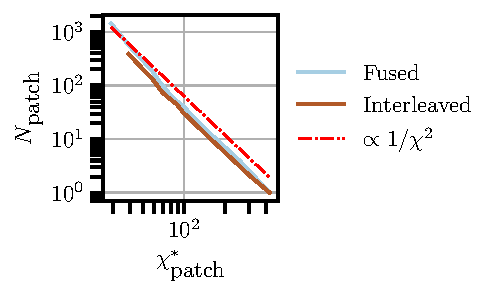
\includegraphics{figures/localFunc_Npatch_vs_Chipatch.pdf}
	\caption{Number of total patches vs largest patch maximum bond dimension $\chip^*$ for the approximation of $f(\boldsymbol{r})$ as in \prettyref{eq:localFunc}. The numerical data is compared with the estimated scaling $1/\chi^2$ (cf. \prettyref{eq:scalingNpatchBonddim}).}
	\label{fig:NpatchvsChipatch}
\end{figure}

\subsection{``Over-patching''}
The bond-dimension cap \(\chip\) is pivotal to the efficiency of patched QTCI: it must be selected so that the resulting approximation is truly more economical than a direct (Q)TCI compression. The bounds in \prettyref{eq:chiPatchBound} supply an initial guideline, but they rely on knowing—or at least estimating—the maximum TT rank \(\chi\) that a standard TCI run would produce.  Such information is often unavailable, and even when \(\chi\) can be inferred (for instance, from a previous but costly TCI attempt), the optimal value of \(\chi_{\text{patch}}\) remains strongly problem-specific.
\prettyref{fig:1DOverpatchingBonddim} illustrates this point with a toy example. 

The target is a piecewise function consisting of an oscillatory segment followed by an exponential tail. The colour map reveals that some ways of partitioning the domain are clearly superior to others. In the bottom row of canvas, where the domain is subdivided too aggressively, the number of resulting patches becomes so large that the overall cost exceeds that of a single, full-domain approximation. Over-patching is particularly problematic for functions whose features are not sharply localised: if we split either the exponential tail or the oscillatory region in half, it is impossible to identify a “simpler” versus “harder” sub–interval, and the extra patches provide no computational benefit. 


\begin{figure}[ht!]
	\centering 
	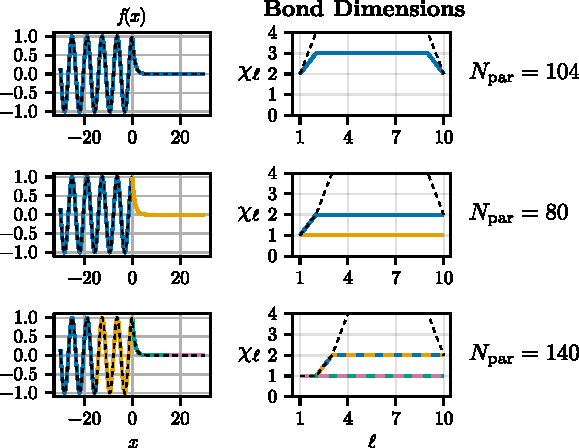
\includegraphics{figures/1DOverpatchingBonddim.pdf}
	\caption{Domain partitioning of a one–dimensional piecewise function and the corresponding bond dimensions of the MPS that represents each segment\protect\footnotemark . Colours link each section of the function (left panels) to the bond dimensions of its TT unfolding (right panels).  \textit{From top to bottom}: a single, global approximation; an optimally subdivided approximation; and an inefficiently over-subdivided case.}
	\label{fig:1DOverpatchingBonddim}
\end{figure}
\footnotetext{I owe a debt of gratitude to my supervisor Marc for this figure.}

This phenomenon—hereafter termed \emph{over-patching}—is common when patched QTCI is applied to functions lacking sharply localised structure, or when the prescribed cap $\chi_{\text{patch}}$ is set too small for the task at hand.  
In either circumstance, once a patch reaches the bond-dimension limit, pQTCI tries to refine the domain further, irrespective of whether the function varies significantly within that patch.  
The outcome is a proliferation of sub-patches whose spatial extent is smaller, yet whose tensor-train representations inherit essentially the \emph{same} bond dimensions as their parent patch, thereby defeating the purpose of the subdivision.



\prettyref{fig:2DOverpatching} shows how patched QTCI can fail when confronted with a function whose features are \emph{uniformly spread across the whole domain}.  
The target here is  
\begin{align}
\label{eq:2Dfunction}
f(x,y) &=
  1
  + e^{-0.4\,(x^{2}+y^{2})}
  + e^{-x^{2}}\sin(xy)
  + e^{-y^{2}}\cos(3xy) \\
  &\quad + \cos(x+y)
  + 0.05\,\cos\!\bigl[10^{2}\,(2x-4y)\bigr] \nonumber\\
  &\quad + 5\!\times\!10^{-4}\,\cos\!\bigl[10^{3}\,(-2x+7y)\bigr]
  + 10^{-5}\,\cos\!\bigl(2\times10^{8}x\bigr), \nonumber
\end{align}
whose oscillatory and exponentially modulated components permeate the entire domain at different length scales.  
Because no subregion is markedly simpler than another, patched QTCI keeps slicing almost at random, generating numerous small patches whose local tensor-train ranks are \emph{identical} to those of their parent regions.  
Consequently, the aggregate number of TT parameters (solid curve in panel~$(b)$) surpasses that of a single, full-domain TCI approximation (dotted curve).  
In effect, the algorithm redundantly stores the same information in multiple MPS blocks, negating any potential savings and exemplifying the drawback of \emph{over-patching}.


\begin{figure}[htbp]
	\centering
	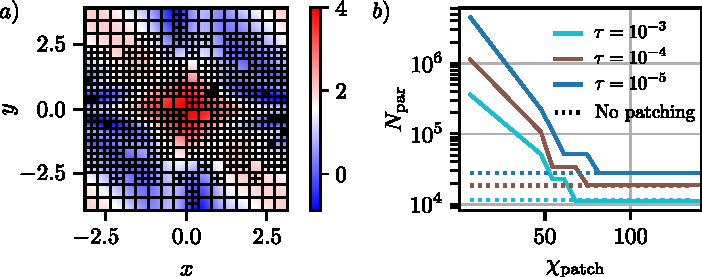
\includegraphics{figures/OverPatching.pdf}
	\caption{Performance of patched QTCI on the two–dimensional oscillatory function of \prettyref{eq:2Dfunction}.  $(a)$ Example of the domain subdivision produced with $\mR = 15$, $\chip = 10$, and $\varepsilon = 10^{-4}$.  The partition is highly redundant and fails to align with the true feature layout of the function. $(b)$ Total number of TT parameters returned by pQTCI (solid curves) at three target tolerances, plotted against the bond-dimension cap $\chip$.  For comparison, the parameter count of a full-domain TCI compression is shown as a dotted line.  Once $\chi_{\text{patch}}\gtrsim 80$, every run collapses to a single patch and matches the TCI cost; for smaller caps, over-patching inflates the parameter count sharply.}
	\label{fig:2DOverpatching}
\end{figure}

To curb over-patching, several practical safeguards could be introduced in future versions of the algorithm
%
\begin{itemize}
  	\item \textbf{Minimum patch size}: impose a lower bound $|\Omega|_{\min}$ on the spatial size of any patch $\Omega_{\mathbf p}$. If a candidate split would produce sub-domains smaller than this threshold, the recursion is halted and the current patch is accepted as is. This solution is particularly useful when the length scales of interest for a target function are known beforehand.
  \item \textbf{Post-processing merge}: after the recursive phase, inspect neighbouring patches whose TT cores share the same effective ranks.  If the error of the combined residual of two siblings stays below $\varepsilon_{\text{merge}}$, replace them by a single, merged patch and recompress with TCI.
\end{itemize}

These mechanisms ensure that domain refinement is driven by actual approximation error rather than the arbitrary attainment of the bond-dimension limit, thereby preventing an explosion in the number of patches and preserving the intended resource savings of patched QTCI.